\documentclass[a4paper,12pt]{article}
\usepackage{cmap}
\usepackage[utf8]{inputenc}
\usepackage[warn]{mathtext}
\usepackage{epsf,amsmath,amsfonts,amssymb,amsbsy}
\usepackage[mathscr]{eucal}
\usepackage[english, russian]{babel}
\author{Мещеряков Павел Б02-920}
\title{Отчёт о выполнении лабораторной работы 2.4.1}
\usepackage[left=2cm,right=2cm,top=2cm,bottom=2cm]{geometry}
\usepackage{graphicx}
\usepackage{indentfirst}
\graphicspath{{pictures2.4.1/}}
\DeclareGraphicsExtensions{.pdf,.png,.jpg}
\usepackage{pgfplots}
\begin{document}
	\maketitle
	\begin{center}
		{\Large Определение теплоты испарения жидкости}
	\end{center}

\paragraph*{Цель работы:} 1) измерение давления насыщенного пара жидкости при разной температуре; 2) вычисление по полученным данным теплоты испарения с помощью уравнения Клапейрона–Клаузиуса.
\paragraph*{В работе используются:} термостат; герметический сосуд, заполненный исследуемой жидкостью; отсчетный микроскоп.

\section{Теоретическое введение}
Теплоту парообразования жидкостей можно измерить непосредственно при помощи калориметра. Такой метод, однако, не позволяет получить точных результатов из-за неконтролируемых потерь тепла, которые трудно сделать малыми. В настоящей работе для определения теплоты испарения применен
косвенный метод, основанный на формуле Клапейрона–Клаузиуса: $$\frac{dP}
{dT} = \frac{L}{T(V_2 - V_1)}\;(1).$$
Здесь $P$ — давление насыщенного пара жидкости при температуре $T$, $T$ — абсолютная температура жидкости и пара, $L$ — теплота испарения жидкости, $V2$ — объем пара, $V1$ — объем жидкости. Найдя из опыта $\frac{dP}{dT},\; T,\; V2$ и $V1$, можно определить $L$ путем расчета. Величины $L, \;V2$ и $V1$ в формуле (1) должны относиться к одному и тому же количеству вещества; мы будем относить их к одному молю.
В нашем приборе измерения производятся при давлениях ниже атмосферного. В этом случае задача существенно упрощается.

С помощью уравнения Ван-дер-Ваальса можно получить зависимость P(T), с помощью которой определить искомую величину:

$$(P+\frac{a}{V^2})(V-b)=RT \; (2)$$
В таблице ниже приведены все значения параметров различных жидкостей уранения Ван-дер-Ваальса в условиях данного опыта.
\begin{figure}[h]
	\center{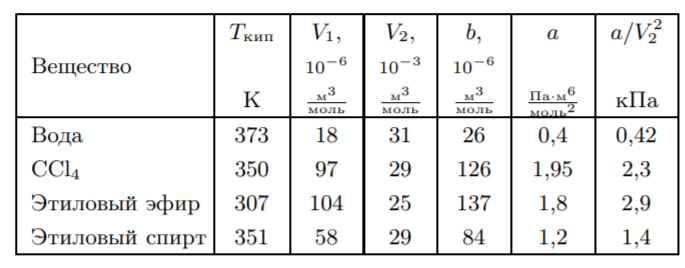
\includegraphics[scale=1]{lab_2_4_1_tablica}}
\end{figure}
Откуда видно, что $\frac{V_1}{V_2} < 0.005$, a $\frac{a}{PV^2}<0.03$, ошибка метода измерений равна 4\%, тогда записав уравнение Клапейрона-Менделеева для насыщенного пара, получим:
$V=\frac{RT}{P}\;.$
Пренебрегая $V_1$ (который не превосходит $0,5\%$ от $V_2$), запишем:
$$L=\frac{RT^2}{P} \frac{dP}{dT} = -R\frac{d(lnP)}{d(1/T)}\;(3).$$
Эта формула является окончательной.
\section{Эксперементальная установка:}

Схема установки изображена на рисунке 1. Наполненный водой резервуар 1 играет роль термостата. Нагревание термостата производится спиралью 2, подогреваемой электрическим током. Для охлаждения воды в термостате через змеевик 3 пропускается водопроводная вода. Вода в термостате перемешивается воздухом,
поступающим через трубку 4. Температура воды измеряетс
я термометром 5. В термостат погружен запаянный прибор 6 с исследуемой жидкостью. Над ней находится насыщенный пар (перед заполнением прибора воздух из него был откачан).
Давление насыщенного пара определяется по ртутному манометру,соединенному с исследуемым объемом. Отсчет показаний манометра производится при помощи микроскопа.


\begin{figure}[h]
	\center{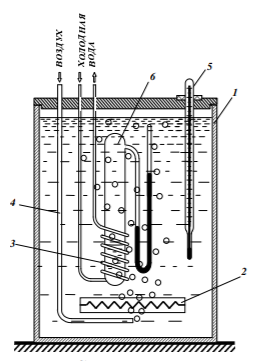
\includegraphics[scale=1.5]{lab_2_4_1_ust}}
	\caption{Схема установки для определения теплоты испарения}
\end{figure}

\section{Ход работы}

\begin{enumerate}
\item Измерим разность уровней в ртутном $U$-образном манометре с помощью микроскопа и температуру по термометру. $H$ - высота высокого колена, $h$ -низкого. При этом будем настраивать микроскоп, так, чтобы каждый раз основание мениска было у метки прибора (в дальнейшем считаем, что высота мениска не меняется, не смотря на то что поверхностное натяжение ртути на самом деле зависит от температуры и высота немного должна меняется). Результаты представлены в таблицах 1 и 2. Под $P_0$ подразумевается давление 1 мм рт.ст.

Приведу формулы для рассчётов погрешностей.
Посколько давление напрямую зависит от разности уровней ртути (пренебрегаем давлением насыщенных паров ртути, так как при комнатной температуре оно приблизительно равно 0.24 Па, а так же изменением уровня столба воды, так как он слишком мал), то
для погрешности давления P воспользуемся следующей формулой: $$ \sigma_P = P_{aтм} \cdot \frac{\sigma_{H-h}}{H_0},$$ где под $H_0$ подразумевается 760 мм, а под $P_{атм} = 101325 \; Па$ - нормальное атмосферное давленине. В качестве $\sigma_{H-h}$ буду брать 2 мм, поскольку, точность измерения каждого из уровня 0.1 мм, а так же мы будем учитывать, что U - образный манометр в нашей установке был не вертикален, а немного наклонён.
$$\sigma_{\ln{\frac{P}{P_0}}} = \frac{\sigma_P}{P} $$

Погрешность определения температуры возьмём учитывая точность прибора и тот факт, что во время измерений уровней температура могла немного изменяться $$\sigma_{T} = 0.2 \; K.$$ Соответсвенно $$\sigma_{\frac{1}{T}} = \frac{\sigma_T}{T^2} \; K^{-1}.$$

\begin{center}
\begin{table}[h]
\begin{tabular}{|c|c|c|c|c|c|c|c|c|c|c|c|}
	\hline 
	$h ,\; {см}$  & 2.91 & 3.53 & 3.30 & 3.24 & 3.18  & 3.00 & 2.95  & 2.78  & 2.61  & 2.55  & 2.47 \\ 
	\hline 
	$H, \; {см}$ & 4.92  & 5.74  & 5.80 & 5.98 & 6.19 &  6.12 & 6.23  & 6.40  & 6.61  & 6.75  &  6.9 \\ 
	\hline 
	$t,\; ^\circ С$ & 22.3 & 24.2 & 25.6 & 26.8 & 28.0 & 29.6 & 31.6 & 33.2 & 34.6 & 35.8 & 37.0 \\
	\hline 
	$P, {кПа}$ & 2.680  & 2.946 & 3.333 & 3.653 & 4.013 & 4.160  & 4.373 & 4.826 & 5.333 & 5.600 & 5.906 \\ 
	\hline 
	$\sigma_{P}, {Па}$  & \multicolumn{11}{|c|}{133}  \\
	\hline 
	$\ln(\frac {P}{P_0})$  & 3.00 & 3.10 & 3.22  & 3.31 &3.41 & 3.44 & 3.49 & 3.59 & 3.69 & 3.74 & 3.79 \\ 
	\hline 
	$\sigma_{\ln(\frac {P}{P_0})}$ & 0.050 & 0.045 & 0.040 & 0.036& 0.033 & 0.032 & 0.030 & 0.028 &0.025  & 0.024 & 0.023 \\ 
	\hline
	$T,\; {K}$ & 295.4 & 297.3 & 298.7 & 299.9 & 301.1 & 302.7 & 304.7 & 306.3 & 307.7 & 308.9 & 310.1 \\
	\hline
	$\sigma_{T},\; {K}$ &\multicolumn{11}{|c|}{0.2} \\
	\hline 
	$\frac{1}{T}$ $\cdot 10^{-3},{K}^{-1}$ & 3.385  & 3.364 & 3.348 & 3.334 & 3.321 & 3.304 &3.282  & 3.265 & 3.250 & 3.237 & 3.224 \\ 
	\hline
	$\sigma_{\frac{1}{T}} \cdot 10^{-6},\; {K}^{-1}$ & 2.292 & 2.263  & 2.242 & 2.223 &  2.206 & 2.183 & 2.154 & 2.132 & 2.113& 2.096 & 2.079 \\
	\hline
\end{tabular}
	\caption{При нагреве}
\end{table}
\end{center}

\begin{center}
\begin{table}[h]
\begin{tabular}{|c|c|c|c|c|c|c|c|c|}
	\hline 
	$h ,\; {см}$ &  3.15 & 3.17 & 2.90 & 2.96 & 2.74 & 2.62 & 2.45 & 2.47    \\ 
	\hline 
	$H, \; {см}$ &  6.12  &6.28  & 6.21 & 6.30 & 6.55 & 6.61 & 6.72 & 6.90    \\ 
	\hline 
	$t, \; ^\circ С$ &  27.4  & 29.0 & 30.0 & 30.6 & 32.6 & 33.8 & 35.0 & 37.0   \\ 
	\hline 
	$P, {кПа}$ &  3.960  & 4.146 & 4.413 & 4.453 & 5.080& 5.320 & 5.693 & 5.906 \\ 
	\hline 
	$\sigma_{P}, {Па}$  & \multicolumn{8}{|c|}{133}  \\
	\hline
	$\ln(\frac {p}{p_0})$ & 3.39  & 3.44 & 3.49 & 3.51 & 3.64 & 3.69 & 3.76 & 3.79 \\ 
	\hline 
	$\sigma_{\ln(\frac {p}{p_0})}$ & 0.034 &  0.032 & 0.030 & 0.030  & 0.026 & 0.025 & 0.023 & 0.023 \\ 
	\hline
	$T , \; {K}$ & 300.5  & 302.1 & 303.1 & 303.7 & 305.7 & 306.9 & 308.1 & 310.1 \\ 
	\hline
	$\sigma_{T},\; {K}$ & \multicolumn{8}{|c|}{0.2} \\
	\hline
	$\frac{1}{T}$ $\cdot 10^{-3},{K}^{-1}$ & 3.328 & 3.310 & 3.299 & 3.293 & 3.271 & 3.258 & 3.246 & 3.225 \\ 
	\hline 
	$\sigma_{\frac{1}{T}} \cdot 10^{-6}, \; {K}^{-1}$   & 2.215  & 2.191 & 2.177 & 2.169 & 2.134 & 2.123 &  2.107 & 2.080 \\ 
	\hline
\end{tabular} 
	\caption{При остывании}
\end{table}
\end{center}


\item Включим термостат. Будем измерять давление и температуру через каждые 1-2 градуса. Продолжим повышать температуру в течение половины имеющегося у нас времени, чтобы успеть произвести измерения при остывании прибора.
\item Проведём те же измерения при охлаждении жидкости.
Установим такой поток воды, чтобы охлаждение шло примерно тем же темпом, что и нагревание.
\item Построим графики в координатах $T$, $P$ и в координатах $\frac{1}{T}, \; ln P$. На графики нанесём точки, полученные при нагревании и охлаждении жидкости. По формуле (3) вычислим $L$, пользуясь данными, полученными  из второго графика.
$L = -R \cdot k,$ где $k$ - коэффициент наклона графика. Итак, $$L_н = 40.3 \pm 1.3 \; \frac{кДж}{моль}, \; L_о = 40.2 \pm 0.9 \; \frac{кДж}{моль}.$$ Погрешности взяты из ошибок в определении коэффициентов фитирующих прямых с помощью МНК. Заметим, что полученные результаты отлично совпадают с теоретическим значением $L_т = 40.7 \; \frac{кДж}{моль}.$ На графике так же заметно, что точки  при остывании расположены выше точек при нагреве. Данный гистерезис можно объяснить следующим образом. Как известно энтропия не убывает, а поскольку в реальности квазистатических процессов не существует, то энтропия растёт. Поэтому система не может возвращаться в исходное состояние по тому же самому пути.
 
 Так же в качестве альтернативного (гораздо менее точного) способа сделаем следкющее: с помощью таблиц 1 и 2 посчитаем $L$ поточечно и усредним (можно конечно было строить график $\frac{1}{P}\frac{dP}{dT}(\frac{1}{T^2})$ и с помощью МНК находить наилучшую прямую, однако эскиз этого графика оставляет желать лучшего и в работе приводить его не будем). Для рассчётов $\frac{dP}{dT}$ пользуемся численным дифференцированием: $$\frac{dP}{dT} \approx \frac{1}{2}\Big(\frac{P(T)- P(T- \Delta T_1)}{\Delta T_1} + \frac{P(T+\Delta T_2)- P(T)}{\Delta T_2}\Big). $$ Результаты представлены в таблицах 3 и 4. 


\begin{table}[h]	
\begin{tabular}{|c|c|c|c|c|c|c|c|c|c|}
	\hline 
	$\frac{dP_н}{dT}, {\frac{кПа}{К}}$  & 0.208 &0.272& 0.257& 0.189& 0.169& 0.214& 0.256&0.257 & 0.234  \\
	\hline 
	$L, {\frac{кДж}{моль}}$  & 51.912 & 60.406 & 52.599 & 36.120 & 30.910 & 36.030 & 40.465 & 37.858 & 33.806  \\
	\hline
\end{tabular}
\caption{Поточечный рассчёт $L$ для нагрева}
\end{table}

\begin{table}[h]
\begin{tabular}{|c|c|c|c|c|c|c|c|c|}
	\hline 
	$\frac{dP_о}{dT}, {\frac{кПа}{К}}$ &0.186 & 0.194& 0.219& 0.244 & 0.239 & 0.202  \\
	\hline
	$L, {\frac{кДж}{моль}}$  & 33.780 & 33.475 & 37.319 & 37.339 & 35.126 & 28.188 \\ 
	\hline
\end{tabular}
\caption{Поточечный рассчёт $L$ для остывания}
\end{table}

\begin{center}
\begin{table}
\begin{tikzpicture}[scale = 1.5]
\begin{axis}[
	axis lines = left,
	legend style={at={(0.9,0.3)}},
	ylabel = {$P, \;  {кПа}$},
	xlabel = {$ T, {К} $},
	xmin=295, xmax=311,
	ymin=2.5, ymax=6,
	ymajorgrids = true,
	xmajorgrids = true,
	yminorgrids = true,
	xminorgrids = true,	
	minor tick num = 4,
	]
	\addplot+[only marks ] plot[error bars/.cd, y dir=both, y explicit]
	coordinates {
		(295.4,2.680) +- (0.1333,0.1333)
		(297.3,2.946) +- (0.1333,0.1333)
		(298.7, 3.333)+- (0.1333,0.1333)
		(299.9, 3.653)+- (0.1333,0.1333)
		(301.1 , 3.95)+- (0.1333,0.1333)
		(302.7, 4.160)+- (0.1333,0.1333)
		(304.7, 4.573)+- (0.1333,0.1333)
		(306.3, 4.926)+- (0.1333,0.1333)
		(307.7, 5.333)+- (0.1333,0.1333)
		(308.9, 5.600)+- (0.1333,0.1333)
		(310.1, 5.906)+- (0.1333,0.1333)
	};
	\addplot+[only marks ] plot[error bars/.cd, y dir=both, y explicit]
	coordinates {
		(300.5,3.96)+- (0.1333,0.1333)
		(302.1,4.176) +- (0.1333,0.1333)
		(303.1, 4.413)+- (0.1333,0.1333)
		(303.7, 4.503)+- (0.1333,0.1333)
		(305.7 , 5.08)+- (0.1333,0.1333)
		(306.9, 5.320)+- (0.1333,0.1333)
		(308.1, 5.653)+- (0.1333,0.1333)
		(310.1, 5.906)+- (0.1333,0.1333)
	};
	\addplot[blue,domain=295:311]{66.4552*ln(0.00352042*x)};
	\addplot[red, domain=295:311]{66.979*ln(0.00352618*x)};
	\legend{
		$нагрев$,$охлаждение$ 
	};
\end{axis}
\end{tikzpicture}
\caption{$P_{н} = -0.375 + 0.0665 \cdot \ln(T)$, $P_{о} =-0.378 + 0.0670 \cdot \ln(T) $}	


	\begin{tikzpicture}[scale = 1.5]
	\begin{axis}[
	axis lines = left,
	legend style={at={(1,0.8)}},
	ylabel = {$\ln{ \frac{P}{P_0}}$},
	xlabel = {$ \frac{1}{T} \cdot 10^{-3},  {К}^{-1} $},
	xmin=3.2, xmax=3.4,
	ymin=3, ymax=4,
	ymajorgrids = true,
	xmajorgrids = true,
	yminorgrids = true,
	xminorgrids = true,
	minor tick num = 4
	]
	\addplot+[only marks ] plot[error bars/.cd, y dir=both, y explicit]
	coordinates {
		(3.385,3.00) +-(0.05,0.05)
		(3.364,3.10) +-(0.045,0.045)
		(3.348, 3.22) +-(0.04,0.04)
		(3.334, 3.31)+-(0.036,0.036)
		(3.321 , 3.37)+-(0.033,0.033)
		(3.304, 3.44)+-(0.032,0.032)
		(3.282, 3.54)+-(0.030,0.030)
		(3.265, 3.61)+-(0.028,0.028)
		(3.250, 3.69)+-(0.025,0.025)
		(3.237, 3.74)+-(0.024,0.024)
		(3.224, 3.79)+-(0.023,0.023)
	};
	\addplot+[only marks ] plot[error bars/.cd, y dir=both, y explicit]
	coordinates {
		(3.328,3.39) +-(0.034,0.034)
		(3.31,3.445) +-(0.032,0.032)
		(3.299, 3.49)+-(0.030,0.030)
		(3.293, 3.52)+-(0.030,0.030)
		(3.271 , 3.64)+-(0.026,0.026)
		(3.258, 3.69)+-(0.025,0.025)
		(3.246, 3.75)+-(0.023,0.023)
		(3.225, 3.79)+-(0.023,0.023)
	};
	
	\addplot[blue, domain=3.2:3.5]{19.474 - 4.85719*x};
	\addplot[red, domain=3.2:3.5]{19.471 - 4.84283 *x};
	\legend{
		$нагрев$,$охлаждение$
		};
	\end{axis}
	\end{tikzpicture}
	\caption{$\ln{\frac{P_н}{P_0}} = (19.5 \pm 0.5) - (4860 \pm 160) \cdot \frac{1}{T}, \; ln{\frac{P_о}{P_0}} =(19.5 \pm 0.4) - (4840\pm 110) \cdot \frac{1}{T}$}
\end{table}
\end{center}

Искать удельную теплоту парообразования $L$ будем по следующим формулам: 
$$\overline{L} = \frac{\sum_{i=1}^{N} L_{i}}{N},\; \sigma_L = \overline{L} \sqrt{\frac{\sum_{i=1}^{N} (\frac{\sigma_{L_{i}}}{L_i})^2}{N} + \frac{\sum_{i=1}^{N} (\frac {L_{i}}{\overline{L}}-1)^2}{N(N-1)}}, L = \overline{L} \pm \sigma_L.$$ Где $\sigma_{L_i} = $ - погрешность определения $i$-ого значения $L$. Основной вклад в определение этой погрешности будет вносить производная $\frac{dP}{dT}$. $\sigma_{L_i} \approx L_i (\sigma_{\frac{dP}{dT}}/\frac{dP}{dT}) \approx L_i \frac{\sigma_P}{\sqrt{2}\Delta P} \approx 0.5 L_i $ 
Поэтому имеет смысл в итоговой формуле учитывать только погрешность производной и говорить не о значении $L$, а лишь о порядке $L$. Итак: $$L_н = 42 \pm 21 \; \frac{кДж}{моль}, \; L_о = 34 \pm 17 \frac{кДж}{моль}.$$

\section{Вывод}
В работе изучалась зависимость давления насыщенного пара воды от температуры. По полученным данным искалась разными способами удельная теплота парообразования воды. Были использованы такие методы, как линеаризация зависимости поточечное дифференцирование графика. На основе полученных результатов можно сделать вывод, о том, что второй способ является лишь оценочным, с его помощью можно получить лишь порядок величины. Первый же метод даёт значение хорошо совпадающее с теоретическим. Эффект необратимости процессов в нашей системе, не очень влияет на окончательный результат.
\end{enumerate}


\end{document}